\chapter{Méthode de Newton Raphson}\label{Ch_NewRaph}\index{méthode de Newton-Raphson}
\begin{abstract}
La méthode de Newton-Raphson\index[aut]{Newton (Isaac, Sir -), 1643-1727, Anglais}\index[aut]{Raphson (Joseph), 1648-1715, Anglais} est, dans son application la plus simple, un algorithme efficace pour trouver numériquement une approximation précise d'un zéro (ou racine) d'une fonction réelle d'une variable réelle. 
\end{abstract}

\medskip
\section{Présentation}

\begin{histoire}%
\sbox{\MaBoiteAvecPhotos}{\setlength{\tabcolsep}{0pt}\scriptsize%
\begin{tabular}{ccc}%
\includegraphics[height=\the\HauteurDesPhotos]{Newton3}&
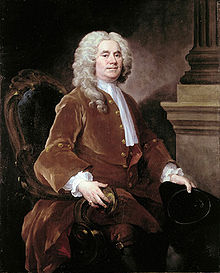
\includegraphics[height=\the\HauteurDesPhotos]{Jones}&
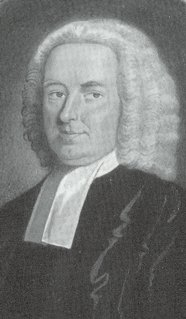
\includegraphics[height=\the\HauteurDesPhotos]{Colson}\\
Newton&Jones&Colson%
\end{tabular}}
\vspace{1mm}~
\ImageADroite{%
La méthode\index{méthode de Newton-Raphson} de Newton\index[aut]{Newton (Isaac, Sir -), 1643-1727, Anglais} fut décrite par Newton dans \emph{De analysi per aequationes numero 
terminorum infinitas}, écrit en 1669 et publié en 1711 par William Jones.\index[aut]{Jones (William, Sir -), 1675-1749, Gallois} Elle fut à nouveau décrite dans \emph{De metodis fluxionum et serierum infinitarum} (De la méthode des fluxions et des suites infinies), écrit en 1671, traduit et publié sous le titre \emph{Methods of Fluxions} en 1736 par John Colson.\index[aut]{Colson (John), 1680-1760, Anglais} Toutefois, Newton\index[aut]{Newton (Isaac, Sir -), 1643-1727, Anglais} n'appliqua la méthode qu'aux seuls polynômes. 
Comme la notion de dérivée et donc de linéarisation n'était pas définie à cette époque, son approche diffère de l'actuelle méthode: Newton\index[aut]{Newton (Isaac, Sir -), 1643-1727, Anglais} cherchait à affiner une approximation grossière d'un zéro d'un polynôme par un calcul polynomial.}

\sbox{\MaBoiteAvecPhotos}{\setlength{\tabcolsep}{0pt}\scriptsize%
\begin{tabular}{cc}%
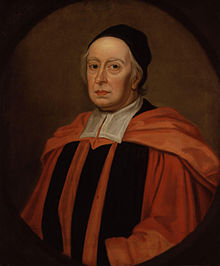
\includegraphics[height=\the\HauteurDesPhotos]{Wallis}&
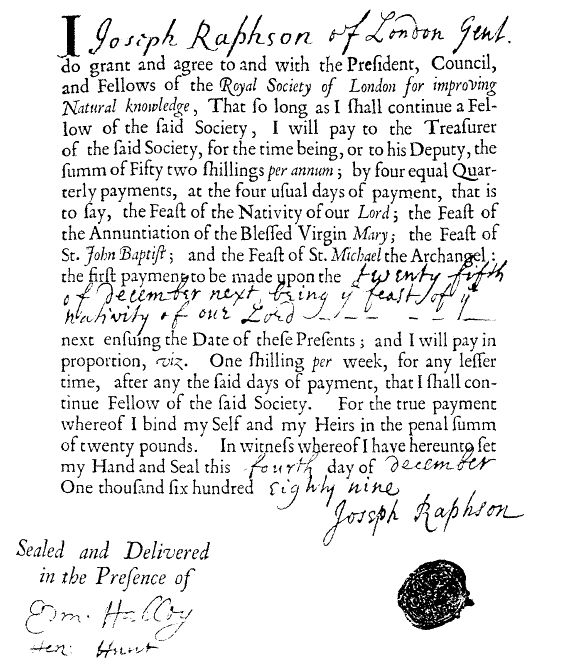
\includegraphics[height=\the\HauteurDesPhotos]{Raphson-manu}\\
Wallis&Raphson%
\end{tabular}}
\medskip
\ImageAGauche{%
Cette méthode fut l'objet de publications antérieures. En 1685, John Wallis\index[aut]{Wallis (John), 1616-1703, Anglais} en publia une première description dans \emph{A Treatise of Algebra both Historical and Practical}. En 1690, Joseph Raphson\index[aut]{Raphson (Joseph), 1648-1715, Anglais} en publia une description simplifiée dans \emph{Analysis aequationum universalis}. Raphson\index[aut]{Raphson (Joseph), 1648-1715, Anglais} considérait la méthode de Newton\index[aut]{Newton (Isaac, Sir -), 1643-1727, Anglais} toujours comme une méthode purement algébrique et restreignait aussi son usage aux seuls polynômes. Toutefois, il mit en évidence le calcul récursif des approximations successives d'un zéro d'un polynôme au lieu de considérer comme Newton\index[aut]{Newton (Isaac, Sir -), 1643-1727, Anglais} une suite de polynômes.}

\sbox{\MaBoiteAvecPhotos}{\setlength{\tabcolsep}{0pt}\scriptsize%
\begin{tabular}{cc}%
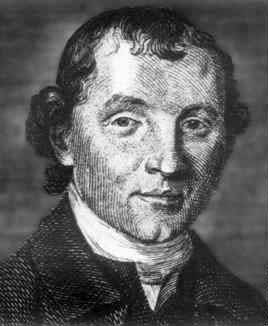
\includegraphics[height=\the\HauteurDesPhotos]{Simpson}&
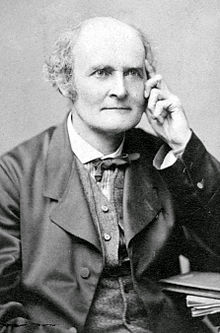
\includegraphics[height=\the\HauteurDesPhotos]{Cayley}\\
Simpson&Cayley%
\end{tabular}}
\medskip
\ImageADroite{%
C'est Thomas Simpson\index[aut]{Simpson (Thomas), 1710-1761, Anglais} qui généralisa cette méthode au calcul itératif des solutions d'une équation non linéaire, en utilisant les dérivées (qu'il appelait fluxions, comme Newton).\index[aut]{Newton (Isaac, Sir -), 1643-1727, Anglais} Simpson\index[aut]{Simpson (Thomas), 1710-1761, Anglais} appliqua la méthode\index{méthode de Newton-Raphson} de Newton\index[aut]{Newton (Isaac, Sir -), 1643-1727, Anglais} à des systèmes de deux équations non linéaires à deux inconnues, en suivant l'approche utilisée aujourd'hui pour des systèmes ayant plus de 2 équations, et à des problèmes d'optimisation sans contrainte en cherchant un zéro du gradient. \\
\indent
Arthur Cayley\index[aut]{Cayley (Arthur), 1821-1895, Anglais} fut le premier à noter la difficulté de généraliser la méthode\index{méthode de Newton-Raphson} de Newton\index[aut]{Newton (Isaac, Sir -), 1643-1727, Anglais} aux variables complexes en 1879, par exemple aux polynômes de degré supérieur à 3.}
\end{histoire}
\colorblack

\medskip
Sous sa forme moderne, l'algorithme se déroule comme suit: à chaque itération, la fonction dont on cherche un zéro est linéarisée en l'itéré (ou point) courant; et l'itéré suivant est pris égal au zéro de la fonction linéarisée. 

Cette description sommaire indique qu'au moins deux conditions sont requises pour la bonne marche de l'algorithme: \textcolorblue{la fonction doit être différentiable} aux points visités (pour pouvoir y linéariser la fonction) et \textcolorblue{les dérivées ne doivent pas s'y annuler} (pour que la fonction linéarisée ait un zéro); s'ajoute à ces conditions la contrainte forte de devoir \textcolorblue{prendre le premier itéré assez proche d'un zéro régulier de la fonction} (i.e. en lequel la dérivée de la fonction ne s'annule pas), pour que la convergence du processus soit assurée.

\medskip
L'intérêt principal de l'algorithme\index{méthode de Newton-Raphson} de Newton-Raphson\index[aut]{Newton (Isaac, Sir -), 1643-1727, Anglais}\index[aut]{Raphson (Joseph), 1648-1715, Anglais} est sa \textcolorblue{convergence quadratique locale}. 
En termes imagés mais peu précis, cela signifie que le nombre de chiffres significatifs corrects des itérés double à chaque itération, asymptotiquement. 
Comme le nombre de chiffres significatifs représentables par un ordinateur est limité (environ 15 chiffres décimaux sur un ordinateur avec un processeur 32-bits), on peut simplifier grossièrement en disant que, soit il converge en moins de 10 itérations, soit il diverge. En effet, si l'itéré initial n'est pas pris suffisamment proche d'un zéro, la suite des itérés générée par l'algorithme a un comportement erratique, dont la convergence éventuelle ne peut être que le fruit du hasard (i.e. si l'un des itérés est par chance proche d'un zéro).

\medskip
L'importance de l'algorithme\index{méthode de Newton-Raphson} de Newton-Raphson\index[aut]{Newton (Isaac, Sir -), 1643-1727, Anglais}\index[aut]{Raphson (Joseph), 1648-1715, Anglais} a incité les numériciens à étendre son application et à proposer des remèdes à ses défauts. 

Par exemple, l'algorithme permet également de trouver un zéro d'une fonction de plusieurs variables à valeurs vectorielles, voire définie entre espaces vectoriels de dimension infinie; la méthode conduit d'ailleurs à des résultats d'existence de zéro. 

On peut aussi l'utiliser lorsque la fonction est différentiable dans un sens plus faible, ainsi que pour résoudre des systèmes d'inégalités non linéaires, des problèmes d'inclusion, d'équations différentielles ou d'équations aux dérivées partielles, d'inéquations variationnelles...

On a également mis au point des techniques de globalisation de l'algorithme, lesquelles ont pour but de forcer la convergence des suites générées à partir d'un itéré initial arbitraire (non nécessairement proche d'un zéro)

Dans les versions dites inexactes ou tronquées, on ne résout le système linéaire à chaque itération que de manière approchée. 

Enfin, la famille des algorithmes de quasi-Newton (par exemple si l'on ne connaît pas l'expression analytique de la fonction dont on cherche une racine) propose des techniques permettant de se passer du calcul de la dérivée de la fonction. 

Toutes ces améliorations ne permettent toutefois pas d'assurer que l'algorithme trouvera un zéro existant, quel que soit l'itéré initial.

\medskip
Appliqué à la dérivée d'une fonction réelle, cet algorithme permet d'obtenir des points critiques (i.e. des zéros de la dérivée). Cette observation est à l'origine de son utilisation en optimisation sans ou avec contraintes.


\medskip
\section{Algorithme}\index{méthode de Newton-Raphson}

Soit~$f: \RR\rightarrow\RR$ la fonction dont on cherche à construire une bonne approximation d'un zéro. pour cela, on se base sur son développement de Taylor\index[aut]{Taylor (Brook), 1685-1731, Anglais} au premier ordre. 

Partant d'un point~$x_0$ que l'on choisit de préférence proche du zéro à trouver (en faisant des estimations grossières par exemple), on approche la fonction au premier ordre, autrement dit, on la considère à peu près égale à sa tangente en ce point:
\begin{equation} f(x)\simeq f(x_0) + f'(x_0)(x-x_0) \end{equation}

Pour trouver un zéro de cette fonction d'approximation, il suffit de calculer l'intersection de la droite tangente avec l'axe des abscisses, i.e. de résoudre:
\begin{equation} 0=f(x_0) + f'(x_0)(x-x_0) \end{equation}

On obtient alors un point~$x_1$ qui en général a de bonnes chances d'être plus proche du vrai zéro de~$f$ que le point~$x_0$ précédent. Par cette opération, on peut donc espérer améliorer l'approximation par itérations successives.

Cette méthode requiert que la fonction possède une tangente en chacun des points de la suite que l'on construit par itération. Cela est évidemment vrai si~$f$ est dérivable.

\medskip
Formellement, on construit donc la suite:
\begin{equation} x_{k+1} = x_k - \frac{f(x_k)}{f'(x_k)} \end{equation}
à partir d'un point~$x_0$.

\medskip
Bien que la méthode soit très efficace, certains aspects pratiques doivent être pris en compte: 
\begin{itemize}
  \item Avant tout, la méthode\index{méthode de Newton-Raphson} de Newton-Raphson\index[aut]{Newton (Isaac, Sir -), 1643-1727, Anglais}\index[aut]{Raphson (Joseph), 1648-1715, Anglais} nécessite que la dérivée soit effectivement calculée. 
	Dans les cas où la dérivée est seulement estimée en prenant la pente entre deux points de la fonction, la méthode prend le nom de \textcolorblue{méthode de la sécante}, moins efficace.
  \item Par ailleurs, si la valeur de départ est trop éloignée du vrai zéro, la la méthode\index{méthode de Newton-Raphson} de Newton-Raphson\index[aut]{Newton (Isaac, Sir -), 1643-1727, Anglais}\index[aut]{Raphson (Joseph), 1648-1715, Anglais} peut entrer en boucle infinie sans produire d'approximation améliorée. 
	À cause de cela, toute mise en œuvre de la méthode de Newton-Raphson doit inclure un code de contrôle du nombre d'itérations.
\end{itemize}


